\chapter{Описание решения}
 {\color{red} Это раздел для декомпозиции задачи и описание Methods для каждой подзадачи   }

 \section{Используемые системы координат   }\label{41}
На данном этапе используются две системы координат: 1-я, связанная с футбольным полем, где левый верхний угол считается точкой (0, 0) и 2-я, связанная с координатами камеры, в системе отсчета, связанной с левым дальним углом поля. Для наперед заданных координат  $X,\;Y$ переход от одной плоскости к другой осуществляется по нижеследующему закону:

$$
\begin{bmatrix}
\tau_{i}X' \\
\tau_{i}Y' \\
\tau_{i}
\end{bmatrix} = 
\underbrace{ \begin{bmatrix}
a_{1} & a_{2} & b_{1} \\
a_{3} & a_{4} & b_{2} \\
c_{1} & c_{2} & 1
\end{bmatrix} }_{ M } \begin{bmatrix}
X \\
Y \\
1
\end{bmatrix},
$$

где $a_i$ это элементы масштабирования/поворота, $\begin{bmatrix}
    b_2 & b_1
\end{bmatrix}^T$ это вектор смещения и $\begin{bmatrix}
    c_1 & c_2
\end{bmatrix}$ это вектор проекции.

Для нахождения истинных значений $X', Y'$ результирующий вектор должен быть поделен на коэффициент $\tau_i$, который является фактором масштабирования. 

В результате был разработан алгоритм, с использованием библиотеки cv2, который принимает на вход 2 аргумента, а именно 4 первоначальные координаты (x, y), которые показывают первоначальные углы прямоугольника захватываемой для перехода области, а также второй аргумент - 4 координаты, которые показывают желаемые угловые координаты для выходной картинки. В результате работы алгоритма получена матрица перехода $M \in \mathbb{R}^{3 \times 3}$, после чего алгоритм последовательно применяется к каждому отдельно взятому кадру из изначально заданного набора данных. В результате, получается новый набор данных, в котором для каждого id, то есть распознанного на кадре объекта, получены новые координаты ($X', Y'$). Пример, визуализирующий работу алгоритма:

 \begin{figure}[!h]
     \centering
     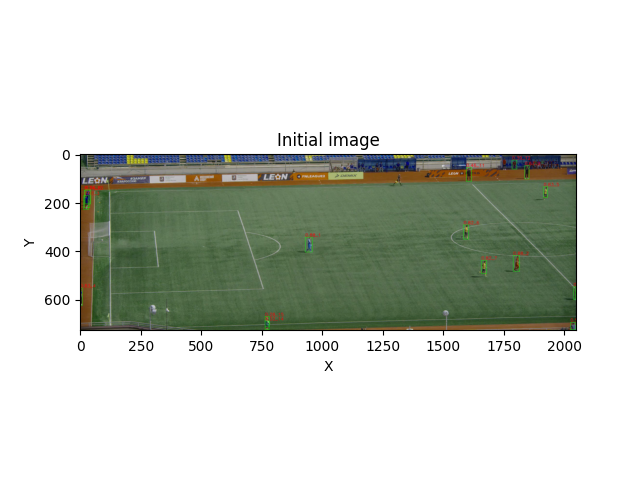
\includegraphics[width=0.8\linewidth]{figures/Initial image.png}
     \caption{Image before transformation of coordinates}
     \label{fig:before-transform}
 \end{figure}

  \begin{figure}[!h]
     \centering
     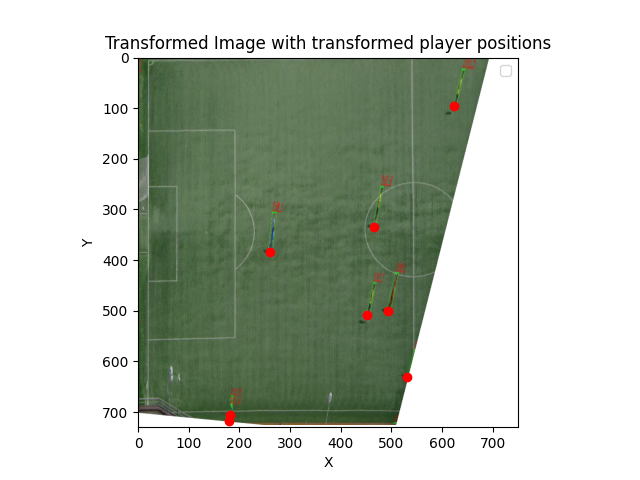
\includegraphics[width=0.8\linewidth]{figures/Transformed Image with transformed player positions.png}
     \caption{Image after transformation of coordinates}
     \label{fig:after-transform}
 \end{figure}


 \section{Предварительная обработка}

 \section{Разработка алгоритма обхода для случая неподвижных игроков   }
Для решения задачи TSP существует множество решений, однако между ними есть ряд ключевых отличий, основным из которых является точность решения. Есть алгоритмы, способные решить задачу нахождения минимального замкнутого пути точно, есть те, что не гарантируют минимальный обход, однако значительно выигрывают в скорости. Для данной конкретной задачи был выбран вариант точного решения, поскольку количество n, то есть количество распознанных на кадре объектов невелико.

Таким образом, согласно статье~\cite{Zhang_2021} наиболее оптимальным вариантом оказался dynamic programming method, поскольку среди точных подходов к решению TSP он показал наибольшую скорость. Реализованный алгоритм принимает на вход один кадр с распознанными объектами, с уже трансформированными координатами, переход к которым был решен в пункте \ref{41}, и возвращает путь, включающий в себя id всех распознанных на кадре объектов, в порядке, который позволяет минимизировать гамильтонов замкнутый путь на графе, вершинами которого являются id, а также сумму пути. Для следующей задачи разработки алгоритма обхода для случая подвижных игроков, вероятно, придется пересмотреть алгоритмический подход к решению задачи, тем не менее dynamic programming подход можно считать успешным на текущем этапе. 

\section{Симуляция Среды}
\subsection{Симуляция агентов}
\subsection{Симуляция камеры}
Пересечение плоскости с прямой:
Пусть $p_0$ - это вектор камеры, а $v_0$ - вектор направления света угловой точки фокальной плоскости, проходящий через вектор камеры (центр фокусного объектива).

Тогда параметрическое уравнение прямой может быть определено как:
$$P(t) = p_0 + t \cdot v_0 \qquad \text{($P(t)$ - точка на прямой)}$$

Нам нужно найти такое $t$, что $P(t)$ лежит на заданной плоскости.
Подставив это в уравнение плоскости, мы получаем:
$$a(P0_x + tV0_x) + b(P0_y + tV0_y) + c(P0_z + tV0_z) = d$$

Решая для $t$ ($n$ - нормальный вектор плоскости):
$$t = \frac{D - nP0}{n \cdot V0}$$

Нас интересует $t < 0$, так как положительные значения соответствуют неправильному направлению света.

\subsubsection{Поле зрения и угол зрения}
Поле зрения:  Метод calculatePanoramicSystemFOV вычисляет угол обзора (FOV) для каждой камеры в
панорамной системе и возвращает список углов обзора камер для панорамной системы.

Метод определяет вектор плоскости и координаты и углы поворота панорамной системы. Затем для каждой камеры в панорамной системе происходит следующее:

    \begin{enumerate}
        \item Вычисляются координаты камеры и ее углы обзора.
        \item Создаются векторы, определяющие углы обзора камеры.
        \item Применяются повороты к векторам камеры и панорамной системы.
        \item Рассчитывается точка пересечения прямой (определяемой камерой) с плоскостью (панорамной системой).
        \item Вычисляется угол обзора камеры и основная ось обзора камеры.
    \end{enumerate}


1. Вычисление вектора vector a:
$$
\text{vector\_a} = \begin{bmatrix}
1.0 \\
\tan\left(\frac{\text{camera\_width\_angle\_of\_view}}{2}\right) \\
-\tan\left(\frac{\text{camera\_height\_angle\_of\_view}}{2}\right)
\end{bmatrix}
$$

2. Поворот вектора $ \mathbf{a} $:
$$
\mathbf{a} = \left(\mathbf{R}_\text{ps} \cdot \mathbf{R}_\text{c}\right) \cdot \mathbf{a}
$$

Здесь $ \mathbf{R}_\text{ps} $ и $ \mathbf{R}_\text{c} $ представляют собой матрицы поворота для панорамной системы и камеры соответственно.

3. Повторный поворот векторов $ \mathbf{b} $, $ \mathbf{c} $, $ \mathbf{d} $, $ \mathbf{p} $:
\begin{align*}
\mathbf{b} &= \left(\mathbf{R}_\text{ps} \cdot \mathbf{R}_\text{c}\right) \cdot \mathbf{b} \\
\mathbf{c} &= \left(\mathbf{R}_\text{ps} \cdot \mathbf{R}_\text{c}\right) \cdot \mathbf{c} \\
\mathbf{d} &= \left(\mathbf{R}_\text{ps} \cdot \mathbf{R}_\text{c}\right) \cdot \mathbf{d} \\
\mathbf{p} &= \left(\mathbf{R}_\text{ps} \cdot \mathbf{R}_\text{c}\right) \cdot \mathbf{p} 
\end{align*}

Здесь $ \mathbf{R}_\text{ps} $ и $ \mathbf{R}_\text{c} $ также представляют собой матрицы поворота для панорамной системы и камеры.

4. Вычисление точки $ \mathbf{t}_0 $:
$$
\mathbf{t}_0 = \mathbf{r}_\text{ps} + \mathbf{R}_\text{ps} \cdot \mathbf{r}_\text{c}
$$

Здесь $ \mathbf{r}_\text{ps} $ и $ \mathbf{r}_\text{c} $ представляют собой координаты панорамной системы и камеры соответственно.
5. Определение параметров $a_0$, $b_0$, $c_0$, $d_0$, $p_0$:

\begin{align*}
a_0 &= -\frac{\left(\mathbf{v}_\text{plane} \cdot \mathbf{v}_{\text{t}_0}\right) + D} {\left(\mathbf{v}_\text{plane} \cdot \mathbf{v}_a\right)} \\
b_0 &= -\frac{\left(\mathbf{v}_\text{plane} \cdot \mathbf{v}_{\text{t}_0}\right) + D} {\left(\mathbf{v}_\text{plane} \cdot \mathbf{v}_b\right)} \\
c_0 &= -\frac{\left(\mathbf{v}_\text{plane} \cdot \mathbf{v}_{\text{t}_0}\right) + D}{\left(\mathbf{v}_\text{plane} \cdot \mathbf{v}_c\right)} \\
d_0 &= -\frac{\left(\mathbf{v}_\text{plane} \cdot \mathbf{v}_{\text{t}_0}\right) + D}{\left(\mathbf{v}_\text{plane} \cdot \mathbf{v}_d\right)} \\
p_0 &= -\frac{\left(\mathbf{v}_\text{plane} \cdot \mathbf{v}_{\text{t}_0}\right) + D}{\left(\mathbf{v}_\text{plane} \cdot \mathbf{v}_p\right)}
\end{align*}

6. Расчет координат углов обзора и основной оси камеры:
\begin{align*}
\text{fov\_a} &= a_0 \cdot \mathbf{v}_a + \mathbf{v}_{\text{t}_0} \\
\text{fov\_b} &= b_0 \cdot \mathbf{v}_b + \mathbf{v}_{\text{t}_0} \\ 
\text{fov\_c} &= c_0 \cdot \mathbf{v}_c + \mathbf{v}_{\text{t}_0} \\ 
\text{fov\_d} &= d_0 \cdot \mathbf{v}_d + \mathbf{v}_{\text{t}_0} \\ 
\text{main\_axis} &= p_0 \cdot \mathbf{v}_p + \mathbf{v}_{\text{t}_0} \\
\end{align*}

Эти преобразования необходимы для вычисления параметров углов обзора и основной оси камеры в панорамной системе. Они осуществляют преобразования координат и векторов, учитывая их начальные положения и повороты относительно системы координат, связанных с панорамной системой. Затем, используя найденные параметры, определяются точки, обозначающие углы обзора каждой камеры, а также точка, представляющая основную ось камеры. Эти шаги позволяют определить положение и направление обзора каждой камеры в контексте панорамной системы.


Угол зрения (Angle of View): 
Этот метод вычисляет вертикальный угол обзора камеры. Рассмотрим математику этого процесса.

Пусть $f$ - фокусное расстояние объектива камеры, $H$ - высота фокальной плоскости камеры. Мы хотим найти вертикальный угол обзора $\theta_{\text{vertical}}$, который позволяет определить, сколько градусов по вертикали охватывает камера.

Используя теорему о подобных треугольниках, мы понимаем, что вертикальный угол обзора можно выразить как двойной арктангенс отношения высоты фокальной плоскости к удвоенному фокусному расстояния:

$$
\theta_{\text{vertical}} = 2 \times \arctan \left( \frac{H}{2f} \right)
$$

Таким образом, мы находим угол, под которым видно изображение на фокальной плоскости относительно центральной оси камеры. Это дает нам представление о том, какая часть вертикального пространства охватывается изображением.

\subsubsection{Определение $\Delta$ крен и $\Delta$ тангаж в процессе перемещения}
Для симуляции камеры и алгоритма в целом важно иметь возможность управлять камерой. 
Для того, чтобы управлять камерой, в нашем исследовании, мы можем отправлять $\Delta \theta$  и $\Delta \phi$ ($\Delta$ крен и $\Delta$ тангаж) изменения в нашу камеру (симулируемую либо реальную). 


1. Центральная точка углов обзора:

   Находим центральную точку между двумя угловыми точками обзора (FOV):

   Пусть  $ P_1  $ и  $ P_2  $ - две угловые точки обзора камеры, тогда центральная точка  $ C  $ будет:

    $$
   C = \left( \frac{P_{1x} + P_{2x}}{2}, \frac{P_{1y} + P_{2y}}{2} \right)
    $$

2. Вычисление угла:

   Рассчитываем угол наклона камеры относительно горизонтали и вертикальный угол обзора камеры:

   Пусть  $ (x_c, y_c)  $ - координаты камеры,  $ (x_i, y_i)  $ - начальная позиция,  $ (x_t, y_t)  $ - целевая позиция. Также  $ h  $ - высота камеры, а  $ \theta_{\text{pitch}}  $ - угол вертикального обзора, $\theta_0$ - угол вертикального наклона в данный момент, $\theta_{\text{top\_aov}}$ - угол между высшим входящим лучем света на фотокамеру и основной оси камеры ($AOV_{\text{vert}}/2$).   

   Для начала определяем угол наклона камеры (yaw), используя векторы направления от камеры к начальной и целевой позициям:

    $$
   \Delta \theta_{\text{yaw}} = \text{atan2}(y_t - y_c, x_t - x_c) - \text{atan2}(y_i - y_c, x_i - x_c)
    $$

   Затем вычисляем угол тангажа (pitch), который представляет собой угол наклона камеры относительно горизонта для:


    $$
   \theta_{\text{pitch}} = 90^\circ - \text{toDegrees}(\arctan( \frac{|(x_t-x_c, y_t-y_c) | }{h}) )
    $$

    $$
   \Delta \theta_{\text{pitch}} = \theta_{\text{pitch}} - \theta_{\text{top\_aov}} - \theta_{0}
    $$

Здесь  $ \text{atan2}  $ - функция арктангенса двух аргументов,  $ \| \cdot \|  $ - норма вектора, а  $\mod$ - операция взятия остатка от деления.




\section{Разработка алгоритма обхода для случая подвижных игроков}
 
 Движение игроков считаем априорно неизвестным. 

\subsection{Master-Route Baseline}
Базовый алгоритм, является прохождением камерой по полю *змейкой*. Камера поочередно осматривает каждую полосу наблюдаемого поля, проходя от левого края поля к правому, а затем от правого края поля к левому. Такая алгоритмика легко реализуется после того как фреймворк из секции 4.4.2 был реализован. Чтобы иплементировать обход по всем игрокам, можно приближать камеру по пути, когда алгоритм определяет, что игрок достаточно близок к его первоначальной територии.


\subsection{Probability-Density-Graphs TSP}
Предположим, что мы знаем граф игроков в момент t. Признаками вершин в такой ситуации будут координаты игроков а также идентификаторы. Обучим алгоритм, который для каждого игрока может по последовательности $[0,t]$ предсказывать вероятностное распределение его позиции (самый простой кейс - 2-мерный гауссиан, то есть стандартное нормальное распределение), тогда можно поставить целью для камеры сфокусироваться на 95\%-ом интервале уверенности в момент t+k, который можно вычислить, используя угловую скорость камеры. Далее камера наводится на вершину так, чтобы была видная вся область с достаточной уверенностью и приближается на конкретного игрока (можно включить здесь линейную интерполяцию его движения). Далее алгоритм повторяется для всех игроков.